%
% matrixoptik.tex
%
% (c) 2019 Prof Dr Andreas Müller, Hochschule Rapperswil
%
\section{Matrixoptik
\label{section:matrixoptik}}
Moderne Kameras verwenden komplexe Linsensysteme mit vielen Linsen
um derart scharfe Bilder zu erzeugen, dass die Pixelgrösse eines
Bildsensors die Auflösung limitiert.
Zum Beispiel ist das Zeiss Otus T$\mathstrut^*$ $55\,\text{mm}$ Objektiv 
eines der schärfsten Objektive auf dem Markt und entsprechend teuer.
Es verwendet 12 Linsen in 10 Gruppen und bildet Punktquellen auf 
Flecke ab, die kleiner als $5\,\mu\text{m}$ sind, also kleiner als
die Pixel eines modernen Sensors.

Die Berechnung solcher optischer Systeme ist eine sehr anspruchsvolle
Aufgabe, die heutzutage mit Computerhilfe erfolgreich gelöst wird.
Für das bereits erwähnt Zeiss Objekt müssen die Krümmungsradien von 20
sphärischen Linsenflächen gewählt werden, die 12 Stärken der Linsen,
sowie die 11 Abstände zwischen den Linsen.
Schliesslich enthält das Design auch einen Linse mit nichtsphärischer
Oberfläche, dessen Form ebenfalls gewählt werden muss.
Dem Designer stehen also über 50 Parameter zur Verfügung, die er
varieren kann, um die genannte erstaunliche Leistung des Objektivs
zu erreichen.

In diesem Abschnitt soll gezeigt werden, wie man mit Hilfe einfacher
Matrizenoperationen ein solches Linsensystem in linearer Näherung,
der sogenannten {\em paraxialen Näherung}, Modellieren und Grössen
wie Brennweite, Vergrösserung oder Farbfehler zu berechnen.

%
% brechungsgesetz.tex
%
% (c) 2019 Prof Dr Andreas Müller, Hochschule Rapperswil
%
\subsection{Das Brechungsgesetz\label{mo:subsection:brechungsgesetz}}
\begin{figure}
\centering
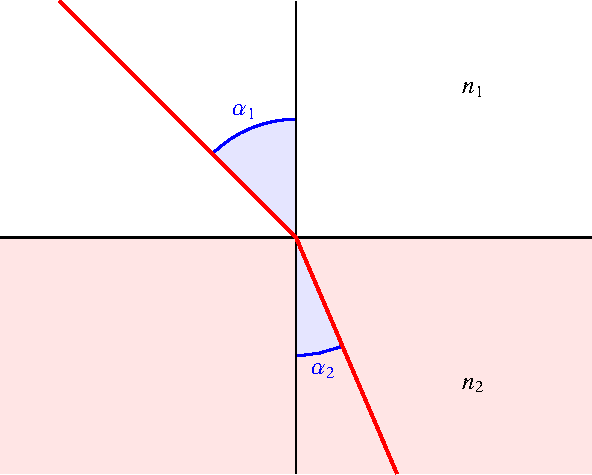
\includegraphics{applications/matrixoptik/snellius.pdf}
\caption{Brechungsgesetz von Snellius
\label{mo:snellius}}
\end{figure}
Das Brechungsgesetz von Snellius beschreibt, wie ein Lichtstrahl beim
\index{Snellius, Brechungsgesetz}
\index{Brechungsgesetz von Snellius}
Eintritt in ein Medium mit einer höheren optischen Dichte gebrochen
wird.
Die {\em optische Dichte} oder {\em Brechungsindex} eines Mediums gibt an,
wie viel langsamer 
\index{optische Dichte}
\index{Brechungszahl}
sich Licht darin bewegt im Vergleich zur Lichtgeschwindigkeit.
Typische optische Glassorten haben einen Brechungsindex zwischen
1.45 und 1.9.

Misst man den Winkel zwischen einem Lichtstrahl und der Normalen auf
die Grenzfläche der Medien wie in Abbildung~\ref{mo:snellius}
dargestellt, dann verhalten sich die Sinus-Werte dieser Winkel
umgekehrt zu den Brechungsindizes, in Formeln
\begin{equation}
\frac{\sin \alpha_1}{\sin\alpha_2} = \frac{n_2}{n_1}.
\label{mo:eq:snellius}
\end{equation}
Der Brechungsindex in Luft ist mit $1.000292$ sehr nahe bei $1$, so
dass für alle praktischen Zwecke der für Luft der Brechungsindex als
$1$ angenommen werden kann.







%
% transfer.tex
%
% (c) 2019 Prof Dr Andreas Müller, Hochschule Rapperswil
%
\subsection{Strahlen und Transfermatrizen
\label{mo:subsection:transfermatrizen}}
Wir möchten den Verlauf eines Lichtstrahls durch ein optisches System
berechnen können.
Im Allgemeinen müssen wir dazu dem Strahl durch das optische System
folgen und an jeder Grenzfläche das Brechungsgesetz anwenden um die
Richtung des Strahls nach dem Durchgang durch die Grenzfläche zu
bestimmen.
Natürlich kann man dazu die Methoden der Vektorgeometrie verwenden,
die in Kapitel~\ref{chapter:orthogonalitaet} entwickelt werden.
Da das Brechungsgesetz nicht linear ist, werden die Gleichungen, die
wir zu lösen haben, sehr kompliziert werden und es ist unwahrscheinlich,
dass wir eine Lösung in geschlossener Form werden finden können.

Um zum Beispiel die Brennweite einer Linse zu berechnen, genügt es jedoch,
Strahlen zu verfolgen, die sehr nahe am Zentrum durch die Linse gehen.
Die auftretenden Brechungswinkel sind dann sehr klein und wir können im
Brechungsgesetz statt des Sinus den Winkel (in Bogenmass) verwenden.
Der Zusammenhang zwischen den Winkeln wird damit linear und es ist 
denkbar, dass sich in dieser Näherung das optische System mit Matrizen
beschreiben lässt.

In der Praxis werden optische Systeme aus Linsen gebaut, die 
sphärische Oberflächen haben.
Solche Linsen sind besonders einfach herzustellen.
Daher können wir uns für die Anwendungen auf rotationssymmetrische
optische Systeme beschränken, wo Linsen auf einer gemeinsamen
optischen Achse montiert sind.
Wir können uns für die beabsichtigte Näherung weiter auf Strahlen
beschränken, die in einer Ebene durch die optische Achse verlaufen.

\subsubsection{Parametrisierung von Strahlen}
\begin{figure}
\centering
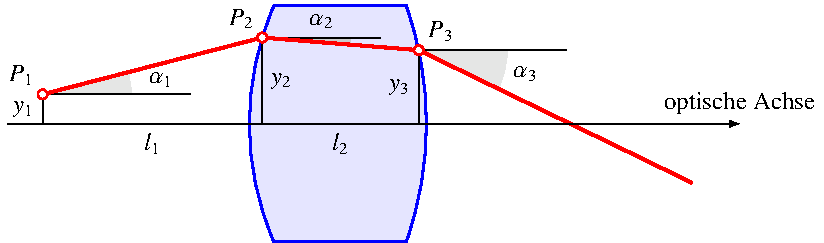
\includegraphics{applications/matrixoptik/ray.pdf}
\caption{Parametrisierung eines Strahls in einem optischen System.
In jedem Punkt wird der Strahl durch den Höhe $y$ über der optischen
Achse und den Winkel $\alpha$ zur optischen Achse beschrieben.
\label{mo:ray}}
\end{figure}
Als erstes müssen wir einen Lichtstrahl im optischen System beschreiben.
In Abbildung~\ref{mo:ray} sind die Punkte hervorgeheben, in denen
die Richtung des Strahls ändert.
Wir können den Strahl rekonstruieren, wenn wir von jedem Punkt den
Abstand $y$ von der optischen Achse kennen sowie den Winkel zur
optischen Achse, unter dem der Strahl den Punkt verlässt.
In der Fachliteratur wird $y$ auch die {\em Höhe} des Strahls über
der optischen Achse genannt.
Den Strahl im Punkt $P_i$ können wir mit dem Vektor
\[
\begin{pmatrix}
y_i\\\alpha_i
\end{pmatrix}
\]
beschreiben.

\subsubsection{Entwicklung entlang der optischen Achse}
Wie hängen die verschiedenen Punkte miteinander zusammen?
Wenn wir dem Strahl, der beim Punkt $P_1$ beginnt, über die Distanz
$l_1$ entlang der optischen Achse folgen, dann ändert sich seine
Höhe über der optischen Achse um $l\sin\alpha_1$.
In der Näherung für kleine Winkel können wir $\sin\alpha_1=\alpha_1$
ersetzen.
Der Winkel des Strahls ändert sich nicht.
Der im Punkt $P_2$ eintreffende Strahl wird also durch den Vektor
\[
\begin{pmatrix}
y_1+l\alpha_1 \\\alpha_1
\end{pmatrix}
\]
beschrieben.
Den Zusammenhang zwischen dem Vektor im Punkt kann durch eine Matrix
beschrieben werden.
Es ist nämlich
\[
\begin{pmatrix}
y_1+l\alpha_1\\\alpha_1
\end{pmatrix}
=
\begin{pmatrix}
1&l\\0&1
\end{pmatrix}
\begin{pmatrix}
y_1\\\alpha_1
\end{pmatrix}
=
T_l
\begin{pmatrix}
y_1\\\alpha_1
\end{pmatrix}
\qquad
\text{mit}
\qquad
T_l
=
\begin{pmatrix}
1&l\\0&1
\end{pmatrix}.
\]

\begin{definition}
Die Matrix
\begin{equation}
T_l
=
\begin{pmatrix}
1&l\\0&1
\end{pmatrix}
\end{equation}
beschreibt also, wie sich ein Strahl über die Distanz
$l$ entwickelt.
\end{definition}

\subsubsection{Brechung}
Im Punkt $P_2$ in Abbildung~\ref{mo:ray} ändert der Strahl seine
Richtung.
Das Brechungsgesetz beschreibt, wie sich der Winkel ändert.
So wie die Matrix $T_l$ den Zusammenhang der den Strahl beschreibenden
Vektoren über die Distanz $l$ wiedergibt, sollte sich auch eine
Matrix finden lassen, welche den Zusammenhang zwischen dem ankommenden
und dem abgehenden Strahl wiedergeben kann.
Diese Matrix wird von den Brechungsindizes $n_1$ und $n_2$ und vom
Krümmungsradius $R$ der brechenden Fläche abhängen, 
\[
\begin{pmatrix}
y_2\\\alpha_2
\end{pmatrix}
=
B(n_1,n_2,R)
T_l
\begin{pmatrix}
y_1 \\ \alpha_1
\end{pmatrix},
\]
$B(n_1,n_2,R)$ ist die gesuchte Matrix.
Da im Brechungsgesetz nur der Quotient $n_2/n_1$ eingeht, sollte das
auch für $B(n_1,n_2,R)$ der Fall sein.

Um eine Formel für $B(n_1,n_2,R)$ herzuleiten, untersuchen wir die
in Abbildung~\ref{mo:Bmatrix} dargestellte Situation.
Ein Lichtstrahl trifft im Punkt $P$ mit einem Winkel $\alpha_1$
auf die brechende Fläche auf und verlässt ihn mit dem Winkel $\alpha_2$.
Die Höhe ist natürlich für den ankommenden und den abgehenden Strahl
gleich: $y=y_1=y_2$.

\begin{figure}
\centering
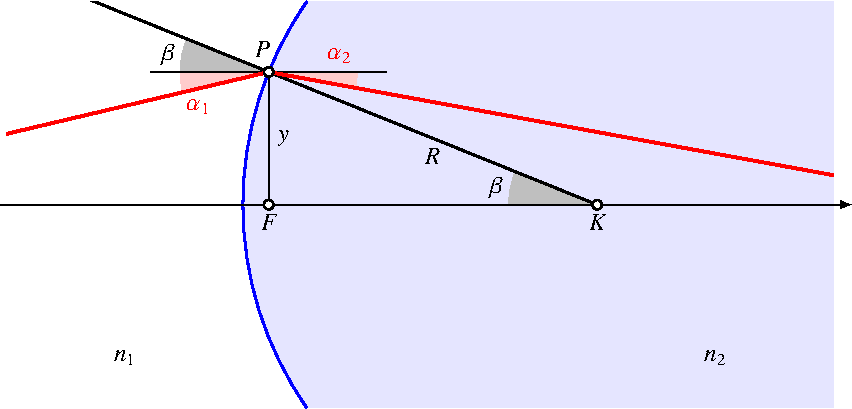
\includegraphics{applications/matrixoptik/curve.pdf}
\caption{Anwendung des Brechungsgesetzes auf die Brechung an einer
sphärischen Fläche.
\label{mo:Bmatrix}}
\end{figure}
Für das Brechungsgesetz sind die Winkel zur Normalen im Punkt $P$
massgebend.
Der Strahl kommt an unter dem Winkel $\beta+\alpha_1$, er verlässt den
Punkt unter dem Winkel $\beta+\alpha_2$ zur Normalen.
Den Winkel $\beta$ können wir im rechtwinkligen Dreieck $\triangle PFK$
ablesen.
Es gilt 
\[
\sin \beta = \frac{y}{R} \simeq \beta.
\]
Das Brechungsgesetz besagt dann
\[
\frac{n_1}{n_2}
=
\frac{\beta+\alpha_2}{\beta+\alpha_1}
\qquad\Rightarrow\qquad
\alpha_2
=
\frac{n_1}{n_2}(\beta+\alpha_1)
-\beta
=
\biggl(
\frac{n_1}{n_2}-1
\biggr)
\frac{y}{R}
+
\frac{n_1}{n_2}\alpha_1
=
\frac{1}{R}
\biggl(
\frac{n_1}{n_2}-1
\biggr)
y
+
\frac{n_1}{n_2}\alpha_1.
\]
Den Zusammenhang zwischen $y_1$, $\alpha_1$, $y_2$ und $\alpha_2$ lässt
sich auch als Matrix schreiben:
\[
\begin{pmatrix}
y_2\\\alpha_2
\end{pmatrix}
=
\begin{pmatrix}
y_1
\\
\displaystyle\frac{1}{R}\biggl(\frac{n_1}{n_2}-1\biggr) y_1
	+ \frac{n_1}{n_2}\alpha_1
\end{pmatrix}
=
\underbrace{
\begin{pmatrix}
1&0\\
\displaystyle\frac{1}{R}\biggl(\frac{n_1}{n_2}-1\biggr)
	& \displaystyle\frac{n_1}{n_2}
\end{pmatrix}
}_{\displaystyle =B(n_1,n_2,R)}
\begin{pmatrix}y_1\\\alpha_1\end{pmatrix}.
\]

\begin{definition}
Die Brechung an einer sphärischen Fläche zwischen Medien mit Brechungsindex
$n_1$ und $n_2$ mit Krümmungsradius $R$ wird beschrieben durch die Matrix
\begin{equation}
B(n_1,n_2,R)
=
B(\nu,R)
=
\begin{pmatrix}
1&0\\
\displaystyle\frac{1}{R}\biggl(\frac{n_1}{n_2}-1\biggr)
	& \displaystyle\frac{n_1}{n_2}
\end{pmatrix}
=
\begin{pmatrix}
1                  & 0  \\
\frac{1}{R}(\nu-1) & \nu
\end{pmatrix}
\label{om:Bn1n2R}
\end{equation}
wobei $\nu = n_1/n_2$ das Verhältnis der Brechungsindizes ist.
\end{definition}

Wie angedeutet hängt $B(n_1,n_2,R)$ nur vom Verhältnis der Brechungsindizes ab.

\subsubsection{Spezialfälle}
Die Matrix $B(\nu,R)$ muss die Brechung an einer Fläche auch in Extremfällen
beschreiben, die wir in diesem Abschnitt untersuchen wollen.

Eine ebene Fläche müsste das Brechungsgesetz reproduzieren.
Eine solche entspricht einem unendlich grossen Krümmungsradius, also
\[
B(\nu,\infty)
=
\begin{pmatrix}
1&0\\0&\nu
\end{pmatrix}.
\]
Diese Matrix besagt, dass
\[
\alpha_2 = \nu \alpha_1 = \frac{n_1}{n_2}\alpha_1
\qquad\Rightarrow\qquad
\frac{\alpha_2}{\alpha_1}=\frac{n_1}{n_2},
\]
dies ist das Brechungsgesetz.

Wenn die Medien auf beiden Seiten der Fläche die gleiche optische
Dichte haben, dann sollte gar keine Brechung stattfinden.
Dies ist der Fall $\nu=1$, in dem die Matrix
\[
B(\nu,R)
=
\begin{pmatrix}
1&0\\
0&1
\end{pmatrix}
\]
die Einheitsmatrix ist, die den Vektor nicht ändert.

\subsubsection{Optische Systeme}
Ein optisches System ist eine Folge von $n$ sphärischen Flächen mit
Krümmungsradius $R_i$, welche Medien mit dem Verhältnis $\nu_i$
der optischen Dichten trennt und an der Position $x_i$ auf der optischen
Achse montiert sind.
Wir verfolgen einen Strahl, der im Punkt $(x_0,y_0)$ mit einem Winkel
$\alpha_0$ abgeht.
Dazu muss jeweils eine Matrix der Form $T_l$ mit $l={x_{i+1}-x_{i}}$
angewendet um zu bestimmen, wie sich der Strahl zwischen den Flächen
$i$ und $i+1$ entwickelt.
An der Fläche $i$ muss die Matrix $B(\nu_i,R_i)$ angewendet werden, um
die Brechung des Strahls zu bestimmen.
Die Wirkung des optischen Systems ist daher gegeben durch die Matrix
\[
T
=
T_{x-x_n}
B(\nu_n,R_n)
T_{x_n-x_{n-1}}
\dots
B(\nu_2,R_2)
T_{x_2-x_1}
B(\nu_1,R_1)
T_{x_1-x_0}.
\]
Sie berechnet wie ein an der Koordinaten $x_0$ auf der optischen Achse
abgehender Strahl an der Koordinate $x$ auf der optischen Achse
ankommt.

In den folgenden Abschnitten soll dieses Prinzip für die Berechnung
einfacher optischer Systeme angewendet werden.





%
% linse.tex
%
% (c) 2019 Prof Dr Andreas Müller, Hochschule Rapperswil
%
\subsection{Dünne Linse\label{mo:subsection:linse}}
Eine Linse besteht aus zwei sphärischen Flächen mit 
Krümmungsradien $R_1$ und $R_2$ (Abbildung~\ref{mo:focus}).
Die Brechungsindexverhältnisse an den beiden Flächen sind reziprok,
also $\nu_2=\nu_1^{-1}$.
Da die Linse als dünn angenommen wird, kann der Abstand der beiden Flächen
vernachlässigt werden, wir nehmen daher $x_1=x_2$ an.

Die Transformatrix des Systems wird daher durch die Matrix
\begin{align*}
T
&=
T_x
B(\nu_2, R_2)
B(\nu_1, R_1)
T_{-x_0}
\\
&=
\begin{pmatrix}
1&x\\
0&1
\end{pmatrix}
\begin{pmatrix}
1&0\\
\frac1{R_2}(\nu^{-1}-1)&\nu^{-1}
\end{pmatrix}
\begin{pmatrix}
1&0\\
\frac1{R_1}(\nu-1)&\nu
\end{pmatrix}
\begin{pmatrix}
1&-x_0\\
0&1
\end{pmatrix}
\\
&=
\begin{pmatrix}
1&x\\
0&1
\end{pmatrix}
\begin{pmatrix}
1&0\\
\frac1{R_2}(\nu^{-1}-1)+\nu^{-1}\frac{1}{R_1}(\nu-1)&1
\end{pmatrix}
\begin{pmatrix}
1&-x_0\\
0&1
\end{pmatrix}
\\
&=
\begin{pmatrix}
1&x\\
0&1
\end{pmatrix}
\begin{pmatrix}
1&0\\
\displaystyle
\biggl(\frac1{R_2}-\frac1{R_1}\biggr)(\nu^{-1}-1)
&1
\end{pmatrix}
\begin{pmatrix}
1&-x_0\\
0&1
\end{pmatrix}
\end{align*}
beschrieben.
Für eine Linse in Luft kann man $n_1=1$ setzen, dann ist $\nu=n_1/n_2$
und damit $\nu^{-1}=n_2$.
Damit ist Transfermatrix
\[
T
=
\begin{pmatrix}
1&x\\
0&1
\end{pmatrix}
\begin{pmatrix}
1&0\\
\displaystyle
\biggl(\frac1{R_2}-\frac1{R_1}\biggr)(n_2-1)
&1
\end{pmatrix}
\begin{pmatrix}
1&-x_0\\
0&1
\end{pmatrix}.
\]

\subsubsection{Brennweite}
\begin{figure}
\centering
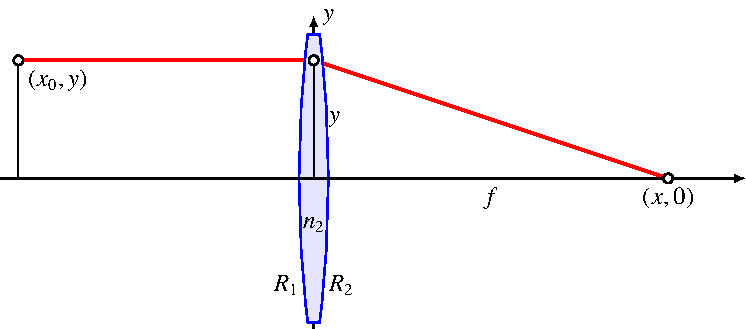
\includegraphics{applications/matrixoptik/fl.pdf}
\caption{Brennweite einer dünnen Linse
\label{mo:focus}}
\end{figure}
Die Brennweite einer Linse ist der Werte $x$, bei dem parallel zur
optischen Achse auf die Linse fallende Strahlen in einem Punkt
zusammenkommen (Abbildung~\ref{mo:focus}).
Ein Strahl parallel zur optischen Achse hat $\alpha_0=0$.
Gesucht wird also dasjenige $x$, für welches der $y$-Wert unter der
Wirkung von $T$ zu $0$ wird:
\begin{align*}
\begin{pmatrix}
0\\?
\end{pmatrix}
&=
T
\begin{pmatrix}y_0\\0\end{pmatrix}
=
\begin{pmatrix}
1&x\\
0&1
\end{pmatrix}
\begin{pmatrix}
1&0\\
\displaystyle
\biggl(\frac1{R_2}-\frac1{R_1}\biggr)(n_2-1)
&1
\end{pmatrix}
\begin{pmatrix}
1&-x_0\\
0&1
\end{pmatrix}
\begin{pmatrix}y_0\\0\end{pmatrix}
\\
&=
\begin{pmatrix}
1&x\\
0&1
\end{pmatrix}
\begin{pmatrix}
1&0\\
\displaystyle
\biggl(\frac1{R_2}-\frac1{R_1}\biggr)(n_2-1)
&1
\end{pmatrix}
\begin{pmatrix}y_0\\0\end{pmatrix}
\\
&=
\begin{pmatrix}
1&x\\
0&1
\end{pmatrix}
\begin{pmatrix}y_0
\\
\displaystyle\biggl(\frac1{R_2}-\frac1{R_1}\biggr)(n_2-1)y_0
\end{pmatrix}
\\
&=
\begin{pmatrix}
y_0 + \displaystyle x\biggl(\frac1{R_2}-\frac1{R_1}\biggr)(n_2-1)y_0
\\
?
\end{pmatrix}.
\end{align*}
Die Brennweite kann gefunden werden, indem man die Gleichung
\[
0=
y_0 + \displaystyle x\biggl(\frac1{R_2}-\frac1{R_1}\biggr)(n_2-1)y_0
\]
nach $x$ auflöst.
Man erhält
\[
x
=
\biggl(
\frac{1}{R_1}-\frac{1}{R_2}
\biggr)^{-1}
(n_2-1)^{-1}.
\]
\begin{satz}
Die Brennweite einer dünnen Linse aus einem Medium mit Brechungsindex $n$ 
mit Krümmungsradien $R_1$ und $R_2$ der Flächen ist
\[
f = \biggl(\frac{1}{R_1}-\frac{1}{R_2}\biggr)^{-1} \frac{1}{n-1}.
\]
\end{satz}

Mit diesem Ausdruck für $f$ kann die Transfermatrix etwas vereinfacht
werden.
Sie lautet
\begin{equation}
T
=
\begin{pmatrix}1&x\\0&1\end{pmatrix}
\begin{pmatrix}1&0\\-f^{-1}&1\end{pmatrix}
\begin{pmatrix}1&x_0\\0&1\end{pmatrix}
\label{om:fokusmatrix}
\end{equation}

\subsubsection{Abbildungsgleichung}
\begin{figure}
\centering
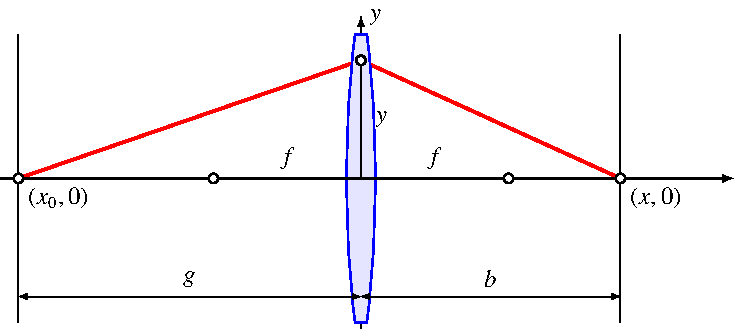
\includegraphics{applications/matrixoptik/abb.pdf}
\caption{Abbildung eines Punktes durch eine dünne Linse.
\label{mo:abb}}
\end{figure}
Wo wird das Licht, welches vom Punkt $x_0$ auf der optischen
Achse ausgeht von einer dünnen Linse fokusiert?

Diese Situation ist in Abbildung~\ref{mo:abb} dargestellt.
Wir betrachten einen Strahl, der vom Punkt $x_0$ 
auf der optischen Achse ausgeht und die Linse auf der Höhe $y$ 
trifft.
Der Winkel zur optischen Achse dieses Strahls ist $\alpha_0=y/x_0$.
Wir suchen also wieder den Punkt $x$ derart, dass der Strahl
wieder durch die optische Achse geht.
Dies bedeutet, dass
\[
\begin{pmatrix} 0\\ y/x \end{pmatrix}
=
T
\begin{pmatrix} 0\\ y/x_0 \end{pmatrix}
\]
sein muss.
Verwenden wir die Form \eqref{om:fokusmatrix} für die Transfermatrix,
erhalten wir die Bedingung
\begin{align*}
\begin{pmatrix}0\\-y/x\end{pmatrix}
&=
T
\begin{pmatrix}0\\ y/x_0\end{pmatrix}
=
\begin{pmatrix}1&x\\0&1\end{pmatrix}
\begin{pmatrix}1&0\\-f^{-1}&1\end{pmatrix}
\begin{pmatrix}1&x_0\\0&1\end{pmatrix}
\begin{pmatrix}0\\ y/x_0\end{pmatrix}
\\
&=
\begin{pmatrix}1&x\\0&1\end{pmatrix}
\begin{pmatrix}1&0\\-f^{-1}&1\end{pmatrix}
\begin{pmatrix}y\\y/x_0\end{pmatrix}
\\
&=
\begin{pmatrix}1&x\\0&1\end{pmatrix}
\begin{pmatrix}y\\ -yf^{-1}+y/x_0\end{pmatrix}
\\
&=
\begin{pmatrix} y-xyf^{-1}+xy/x_0\\ -yf^{-1}+y/x_0 \end{pmatrix}.
\end{align*}
Die erste Komponente dieser Gleichung ist
\begin{align}
0&= y-xyf^{-1}+xy/x_0.
\notag
\intertext{Dividiert man dies durch $xy$ und bringt $f^{-1}$ auf die linke
Seite findet man}
\frac{1}{f}
&=
\frac1x +\frac{1}{x_0}.
\label{om:abbildungsgleichung}
\end{align}
Die zweite Komponente stimmt automatisch überein, wenn 
\eqref{om:abbildungsgleichung} erfüllt ist.
Die Gleichung
\eqref{om:abbildungsgleichung} heisst die {\em Abbildungsgleichung}
einer Linse mit der Brennweite $f$.
Sie besagt, dass ein Objekt im Abstand $-x_0$ von einer Linse mit Brennweite
$f$ fokusiert wird im Abstand $x$ von der Linse.

\begin{satz}
Eine dünne Linse mit Brennweite $f$ bildet einen Gegenstand in der Entfernung
$g$, der {\em Gegenstandsweite}, vor der Linse in einem Punkt im Abstand $b$,
der {\em Bildweite}, hinter der Linse scharf ab, wenn die Abbildungsgleichung
\[
\frac1f = \frac1g + \frac1b
\]
gilt.
\end{satz}


%
% achromat.tex
%
% (c) 2019 Prof Dr Andreas Müller, Hochschule Rapperswil
%
\subsection{Achromat\label{mo:subsection:achromat}}
Die meisten Medien brechen Licht unterschiedlicher Wellenlängen
verschieden stark.
Bei einer einzelnen Linse führt dies dazu, dass die Farben
verschieden grosse Brennweite haben.
Dies führt zu unschönen Farbsäumen und unscharfer Abbildung.

Die Abhängigkeit der Brechkraft von der Wellenlänge heisst {\em Dispersion}.
\index{Dispersioin}
Es gibt zwar auch Gläser mit sehr geringer Dispersion, doch sind diese
leider sehr teuer in der Herstellung und zum Teil auch empfindlich
auf Umwelteinflüsse.
Calzium-Fluorit zum Beispiel hat fast verschwindende Dispersion, darf
aber keinen grossen Temperaturveränderungen ausgesetzt werden.
Es wird daher nur in Spezialanwendungen eingesetzt, zum Beispiel bei
der Masken-Belichtung in der Chip-Herstellung oder für hochwertige 
Astrographen.

Da es Gläser ganz unterschiedlicher Dispersion gibt, besteht die Hoffnung,
durch Kombination geeigneter Gläser in einem mehrlinsigen System zu
erreichen, dass die Farben rot und blau die gleiche Brennweite haben.
Die Farbe grün dazwischen kann dann auch nicht allzu weit weg sein.
Auf diese Art erhält man ein System mit deutlich schwächeren Farbrändern
und grösserer Bildschärfe.

Das einfachste solche System ist der Achromat, erfunden vom  englischen
Amateuroptiker Chester Moor Hall 1733.
Eine Sammellinse aus Kronglas wird mit einer Zerstreuungslinse aus
Flintglas zusammengefügt.
Es entsteht ein System mit drei gekrümmten Flächen, deren Abstand
in begrenztem Rahmen gewählt werden kann.
Es stehen also insgesamt fünf Parameter zur Verfügung, die so gewählt
werden müssen, dass rotes und grünes Licht die gleiche Brennweite
erhalten.




